\documentclass{article}

\usepackage{amsmath, amsthm, amssymb, amsfonts}
\usepackage{thmtools}
\usepackage{graphicx}
\usepackage{setspace}
\usepackage{geometry}
\usepackage{float}
\usepackage[hidelinks]{hyperref}
\usepackage[utf8]{inputenc}
\usepackage[spanish]{babel}
\usepackage{framed}
\usepackage[dvipsnames]{xcolor}
\usepackage{tcolorbox}
\usepackage{tikz}
\usepackage{caption}
\usepackage{longtable}
\usepackage{pdflscape}
\usepackage{svg}
\usepackage{subcaption}
\usepackage{caption}
\usepackage{multirow}
\usepackage{array}
\usepackage{listings}
\usepackage{cancel}
\usepackage{xurl}
\usepackage{pdfpages}

\colorlet{LightGray}{White!90!Periwinkle}
\colorlet{LightOrange}{Orange!15}
\colorlet{LightGreen}{Green!15}



\newcommand{\HRule}[1]{\rule{\linewidth}{#1}}

\declaretheoremstyle[name=Theorem,]{thmsty}
\declaretheorem[style=thmsty,numberwithin=section]{theorem}
\tcolorboxenvironment{theorem}{colback=LightGray}

\declaretheoremstyle[name=Proposition,]{prosty}
\declaretheorem[style=prosty,numberlike=theorem]{proposition}
\tcolorboxenvironment{proposition}{colback=LightOrange}

\declaretheoremstyle[name=Principle,]{prcpsty}
\declaretheorem[style=prcpsty,numberlike=theorem]{principle}
\tcolorboxenvironment{principle}{colback=LightGreen}

\newcolumntype{L}[1]{>{\raggedleft\let\newline\\\arraybackslash\hspace{0pt}}m{#1}}
\newcolumntype{C}[1]{>{\centering\let\newline\\\arraybackslash\hspace{0pt}}m{#1}}
\newcolumntype{R}[1]{>{\raggedright\let\newline\\\arraybackslash\hspace{0pt}}m{#1}}

\setstretch{1.2}
\geometry{
    textheight=9in,
    textwidth=5.5in,
    top=1in,
    headheight=12pt,
    headsep=25pt,
    footskip=30pt
}


% ------------------------------------------------------------------------------

\setlength{\parskip}{3mm}


\begin{document}
% ------------------------------------------------------------------------------
% Cover Page and ToC
% ------------------------------------------------------------------------------

\title{ \normalsize \textsc{}
	\\ [2.0cm]
	\HRule{1.5pt} \\
	\LARGE \textbf{\uppercase{Propuesta Maratón de Programación UTADEO}
		\HRule{2.0pt} \\ [0.6cm] \Large{Sementation Fault, Semillero de Programación Competitiva\\Y\\ GNUTADEO, Colectivo de Software Libre} \vspace*{10\baselineskip}}
}
\date{}
\author{\textbf{Alvarado Becerra Ludwig} \\
	\today}

\maketitle
\thispagestyle{empty}
\newpage
{
\setlength{\parskip}{0pt}  % Reset spacing temporarily
\tableofcontents
\listoffigures
\listoftables
}


\thispagestyle{empty}
\newpage
\setcounter{page}{1}



Los contenidos de este documento están sacados de  ``Aplicación para la Solicitud de Recursos Informáticos''\cite{moreno2006aplicacion}

\section{Resumen}

\section{Introducción}

\subsection{Justificación de la actividad}

Durante los últimos años, la participación de la Universidad Jorge Tadeo Lozano en competencias de programación a nivel nacional ha sido limitada y con resultados poco satisfactorios como se presentan en el cuadro \ref{tab:resultados-competencias} donde el mejor resultado es de la competencia del año 2020 quedando de sexta posición. Sin embargo, a lo largo del tiempo la universidad siempre ha tenido unos resultados bajos. Esta situación ha evidenciado una debilidad significativa en la formación de habilidades en programación competitiva entre los estudiantes de la institución, lo cual impacta directamente en la visibilidad y reputación académica.

\begin{table}[h]
  \centering
  \begin{tabular}{|c|c|c|}
    \hline
    Edición de la competencia& Posición de los equipos de la U& Total de equipos nacional \\ \hline
    XXXI (2017) & 80 & 120 \\ \hline
    XXXII (2018) & 74, 75 & 116 \\ \hline
    XXXIII (2019) & 42, 53, 61, 94 & 119 \\ \hline
    XXXIV (2020) & 6, 19 & 27 \\ \hline
    XXXV (2021) & 58, 60 & 83 \\ \hline
    XXXVI (2022) & 52, 52 & 104 \\ \hline
    XXXVII (2023) & 61 & 106 \\ \hline
    XXXVIII (2024) & 75 & 119 \\ \hline
  \end{tabular}
  \caption{Clasificación de los diferentes equipos representando a la universidad en las ediciones de la Maratón Nacional de Programación ACIS REDIS\cite{icpc2024,icpc2023,icpc2022,icpc2021,icpc2020,icpc2019,icpc2018}}
  \label{tab:resultados-competencias}
\end{table}


Debido a esta problemática, desde hace unos meses se ha iniciado la conformación de un Semillero de Programación Competitiva\cite{pcutadeo_github}, con el objetivo de fortalecer las competencias algorítmicas, lógicas y de trabajo en equipo entre los estudiantes interesados en esta área. Sin embargo, dado que el semillero se encuentra en una etapa inicial, es fundamental complementar su desarrollo con actividades que promuevan la práctica constante, el aprendizaje colaborativa, la motivación a través de la competencia y la captura de nuevos talentos entre los estudiantes.

En este contexto, la Maratón de Programación se plantea como una estrategia clave para fomentar el interés en la programación competitiva, identificar talentos emergentes, y preparar de manera más sólida a los estudiantes para futuras participaciones en competencias regionales y nacionales. Además, esta actividad permitirá consolidar el semillero como un espacio activo y retador, capaz de generar una cultura de excelencia técnica y compromiso académico.

La maratón servirá no solo como una experiencia formativa y evaluativa, sino también como un evento integrador que potencie la comunidad académica en torno a la programación, creando las bases para un mejor desempeño institucional en los rankings de competencias tecnológicas en los próximos años.

\subsection{Objetivos}

\subsubsection{General}

Diseñar e implementar una Maratón de Programación interna en la Universidad Jorge Tadeo Lozano como estrategia formativa y competitiva que permita fortalecer el Semillero de Programación Competitiva, mejorar el desempeño institucional en competencias nacionales, y promover una cultura de excelencia técnica entre los estudiantes.

\subsubsection{Específicos}

\begin{itemize}
  \item Fomentar el interés y la participación estudiantil en actividades de programación competitiva, especialmente entre aquellos que aún no hacen parte del semillero.
  \item Contribuir a la mejora del rendimiento institucional en futuras competencias, mediante el entrenamiento competitivo y la selección temprana de equipos representativos.
  \item Simular las condiciones reales de las competencias nacionales, familiarizando a los estudiantes con las dinámicas, el formato y la presión de tiempo propios de eventos como la Maratón Nacional ACIS REDIS.
  \item Identificar estudiantes con habilidades sobresalientes en lógica, algoritmos y resolución de problemas, para integrarlos y fortalecer la base del semillero.
\end{itemize}


\subsection{Ámbito}


Esta propuesta se desarrolla en el ámbito de las ciencias de la computación, específicamente en el campo de la programación competitiva y la formación en resolución algorítmica de problemas. La actividad se enmarca dentro de los procesos de enseñanza del programa de Ingeniería de Sistemas como se puede ver en los objetivos específicos de formación ``Aplicar los principios de la ciencia de la computación y las matemáticas para lograr soluciones efectivas a los problemas de desarrollo de software utilizando herramientas de programación.''\cite{utadeo_sistemas}. Además, está estrechamente vinculada a asignaturas como fundamentos de programación, algoritmos y programación, estructuras de datos y programación avanzada.

Además, la maratón propuesta trasciende lo meramente académico al insertarse en un contexto de competencias extracurriculares de carácter nacional, articulando la formación técnica con el desarrollo de habilidades como el trabajo en equipo, la toma de decisiones bajo presión, la lógica matemática y el pensamiento crítico. De esta manera, se integra tanto en el plan de estudios como en los procesos de fortalecimiento institucional para la participación en eventos académicos de alto nivel.


\subsection{Descripción general}

En términos generales, esta actividad se trata de que el semillero de programación competitiva y el colectivo de software libre GNUTADEO, organicen y dirijan una competencia de programación competitiva en la universidad utilizando infraestructura del laboratorio de redes y el aplicativo DOMjudge\cite{domjudge-docs}, mismo que utilizan en las competencias del ICPC\cite{domjudge-about}. En este documento se presenta la documentación técnica de cómo se realizará el evento, la infraestructura que se necesitará y toda la metodología empleada.


La fase inicial será de configuración del aplicativo en el servidor de la universidad hecho principalmente por los estudiantes Ludwig Alvarado y Juan José Martínez, miembros del colectivo de sotware libre GNUTADEO. En esta etapa se configura todo el software para que pueda ser llevado el evento; \textit{pullear} las imágenes de Docker\cite{domjudge-judgehost,domjudge-domserver}, configuración del usuario administrador, jurado, equipos, usuarios y \textit{globero}\footnote{Equipo que reparte los globos a los equipos participantes en la competencia que resuelvan problemas}.


A la par que se desarrolla la fase de infraestructura, el semillero de programación competitiva a cargo del profesor José Alejandro Franco Calderón prepararán un conjunto de problemas a resolver durante la competición. Estos problemas van a estar divididos de manera general en dos temáticas; técnicos o algorítmicos prácticos, donde se tengan entradas y salidas bien definidas y donde el enfoque es la implementación directa de estructuras de datos y algoritmos clásicos\footnote{Tenga como ejemplo la plataforma \url{www.leetcode.com}\cite{leetcode} en el que los problemas son muy directos, e.j, ``Invierta una lista enlazada''}; competencia algorítmica o de pensamiento lógico-algorítmico, en estos problemas se introduce un componente narrativo o con mucho contexto y se requiere identificar qué estructuras de datos y algoritmos utilizar, los tipos de soluciones deben ser más creativas y estratégicas\footnote{El ICPC es un buen ejemplo de los problemas, otras plataformas pueden ser: \url{ https://codeforces.com/ }, \url{https://onlinejudge.org/} y \url{https://open.kattis.com/}. }.


Una vez se tengan listos los problemas, se empieza con la fase de divulgación e inscripción. En esta parte se realiza un formulario por medio de Microsoft Forms que esté abierto a toda la comunidad de estudiantes Tadeístas sin importar el semestre ni carrera que esté cursando, aunque el foco principal van a ser estudiantes de la Facultad de Ciencias Naturales e Ingeniería. En el formulario se va a poder elegir el rol que se desea emplear durante la competencia; voluntario de logística, encargado de ayudar con la organización del evento, monitorear que los equipos no se salten las normas y ayudar en cualquier inquietud para estos mismos; por otra parte, se va a tener al participante o competidor, encargado de inscribir el grupo de 3 estudiantes con sus respectivos datos personales (nombres, programa académico y semestre) junto con el nombre del equipo. La divulgación se va a realizar mediante salóneo, grupos de WhatsApp, redes sociales, correo electrónico y con ayuda del voz a voz.


Ya una vez se tenga todo listo, la competencia empieza el sábado de la primera semana del semestre 2025-2S, es decir, el día 26 de julio\cite{utadeo_calendario} a las trece horas hasta las diecinueve horas del día, en total 6 horas de competencia, la primera media hora va a ser para que los participantes entiendan la metodología que se va a manejar durante la competencia, las siguientes cuatro horas y media serán de competencia, por último, la media hora restante será para los ganadores y mostrar los resultados. Para el inicio de la competencia ya se deben tener los equipos registrados en el aplicativo y disponer de los equipos a utilizar por los competidores listos para ser usados por los equipos.


Una vez finalizada toda la jornada de la competencia, se compartirán los resultados con profesores del área de Industrias y Tecnologías Digitales. Las estadísticas serán tanto de la competencia general, como de los equipos individuales, se compartirán; número total de envíos, envíos aceptados, problemas intentados/resueltos, equipos que intentaron/resolvieron cada problema, contador de envíos, uso de lenguajes de programación, porcentaje de envíos correctos, entre otros. Esto será de gran utilidad para identificar en qué problemas son los que más presentan dificultades los alumnos, al compartirse con los profesores ellos pueden ajustar las metodologías y actividades de la clase para poner cubrir estos huecos en los estudiantes.


Por último, se compartirá una encuesta de satisfacción a los participantes para recibir retroalimentación de posibles mejoras en el evento. Aquellos equipos y/o estudiantes que demuestren tener un nivel destacado en la competencia van a ser invitados a formar parte del Semillero de Programación Competitiva, Segmentation Fault. Así, van a tener la oportunidad de poder representar a la universidad en competencias externas a la universidad, fortaleciendo el nivel de la institución y aumentando la pertenencia de los estudiantes a la misma.


\subsection{Metodología y etapas}




\subsection{Planificación de la actividad}

\subsection{Actividad que se ofrece}

\section{Herramientas tecnológicas}

Se va a utilizar como referencia el documento de ``UTADEO - Ficha técnica servidores'' que se encuentra en la sección \ref{sec:anexos} de anexos. Este documento contiene las específicaciones técnicas de los equipos que se encuentran en el laboratorio de redes, el documento (según la \textit{metadata}) es de la fecha 4 de junio de 2025, tener en cuenta que pueden haber actualizaciones debido a las fechas de redacción. Si desea verificar la fecha que se afirma en este documento, puede visitar el repositorio de \textit{GitHub} del documento \href{https://github.com/SegmentationFaultUtadeo/PropuestaMaratonUtadeo/blob/main/Bibliografia/FichaTecnica.pdf}{\textbf{aquí}}, descargar el pdf e inspeccionar la \textit{metadata} del documento (comando \texttt{exiftool}\cite{exiftool}). A su vez, se toma en cuenta los equipos y espacios que cuenta actualmente la universidad.


\subsection{Elementos a considerar}

Para los equipos del laboratorio de redes se va realiza la solicitud tomando en cuenta la documentación oficial del aplicativo DOMjudge\cite{domjudge-docs}.

\begin{itemize}
  \item En primer lugar, se necesita del equipo Hewlett Packard Enterprise STNS 2154 debido a las especificaciones de la máquina y a que cuenta con un sistema operativo Ubuntu Server 20.04. Se requiere de este equipo debido a la participación de múltiples usuarios conectados al mismo tiempo, por lo tanto, el hardware del equipo es perfecto para esto. Además, en la documentación del aplicativo se recomienda tener un equipo GNU/Linux preferiblemente Debian o alguno de sus derivados, en este caso, Ubuntu.
  \item Para este equipo se requiere de abrir los puertos \(80\) y \(3306\). Esto para permitir el tráfico HTTP y el de la base de datos MariaDB. Según el documento anexo estos puertos se encuentran actualmente cerrados.
  \item Se va a realizar la instalación (si es necesaria) de los compiladores de los lenguajes de programación; Java 17\cite{oracle-java} o 21, GCC\cite{gcc} (para C/C++) y el interprete de Python\cite{python-downloads}. Estos son los lenguajes que van a estar disponible para los equipos, por lo tanto, se necesita de sus compiladores.
\end{itemize}

Los computadores que van a utilizar los equipos serán los del módulo 2 y 7A. Para los equipos se requiere:

\begin{itemize}
  \item Los equipos deben organizarse de una manera similar a la que se encuentra en la figura \ref{fig:sala-equipos}, cada equipo va a estar al frente de 3 computadores de los cuales únicamente el del medio debe estar prendido, los otros deben permanecer apagados durante la competencia. Si por algún motivo, el computador asignado no funciona, entonces se puede cambiar a los otros dos disponibles. Los voluntarios que ayuden a la organización del evento se encargarán de vigilar que solo se utilice uno de los computadores por equipo, de lo contrario, los estudiantes participantes serán descalificados.

        \begin{figure}[h]
          \centering
          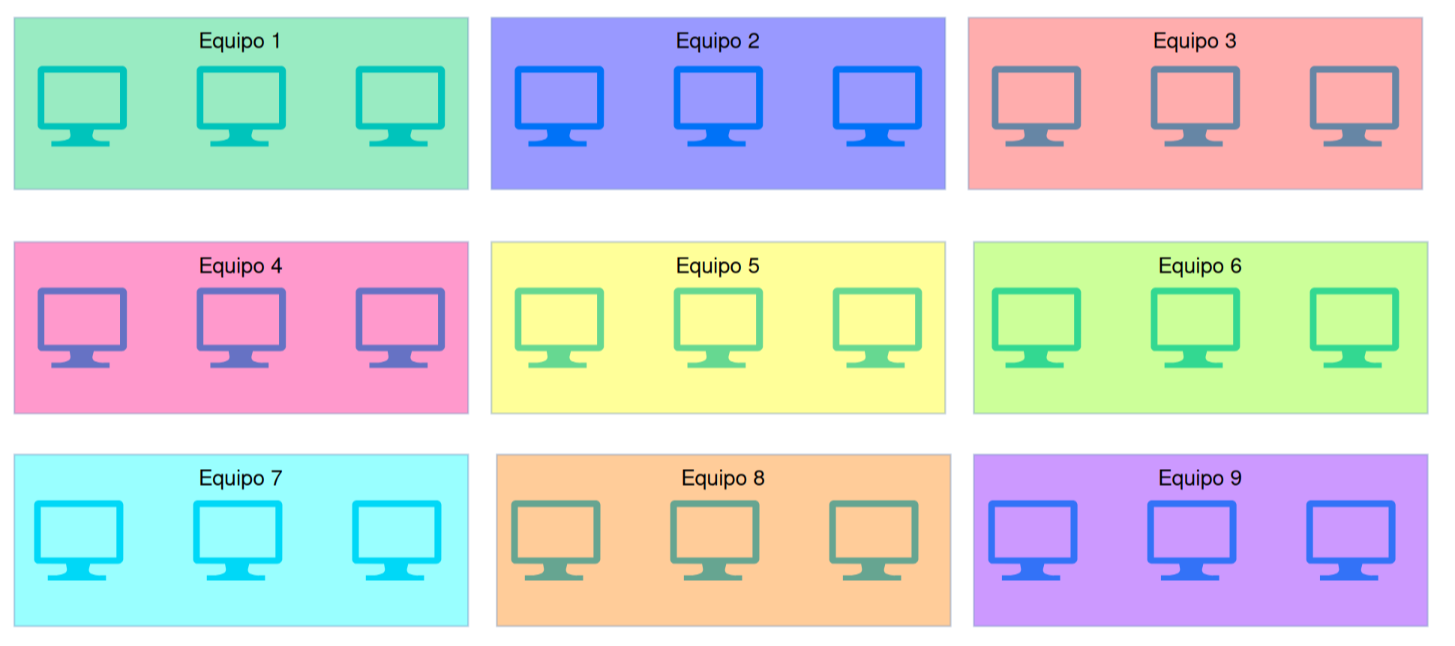
\includegraphics[width=\textwidth]{Assets/Equipos.png}
          \caption{Ejemplo de la organización de equipos en un salón de cómputo }
          \label{fig:sala-equipos}
        \end{figure}
  \item Tener los lenguajes de programación: Java 17 o 21, C/C++ compilador GCC versión 13.2, Python versión \(>=\) 3.9.
  \item IDEs:
        \begin{itemize}
          \item Eclipse versión 4.33.0 configurado con:
                \begin{itemize}
                  \item Java Development Tooling JDT versión 3.19.600.v20240903-0240 y que use el Java que está listado arriba.
                  \item C++ Development Tooling CDT versión 11.0.0 usando C++ mencionado arriba.
                  \item PyDev Python Development Tooling version 10.0.2 usando Python3 listado arriba.
                \end{itemize}
          \item IntelliJ IDEA community versión 2024.2.3 configurado con Java como se lista arriba.
          \item CLion versión 2024.2.2 con GCC listado arriba.
          \item Pycharm community versión 2024.2.3 configurado con Python3 listado arriba.
          \item VS Code versión 1.93.1 configurado únicamente con Python3 y C/C++ listado arriba.
        \end{itemize}
  \item Cualquiera de los siguientes navegadores web:
        \begin{itemize}
          \item Firefox.
          \item Google Chrome.
          \item Microsoft Edge.
        \end{itemize}
\end{itemize}


\section{Análisis de requerimientos}

\subsection{Flujo de trabajo general}

\subsection{Inscripción a la competencia}

\subsection{Aceptación de equipos}

\subsection{Creación de equipos}

\subsection{Ejecución de la actividad}

\subsection{Resultados y premiación}

\subsection{Valoración de la actividad}

\subsection{Estadísticas}

\section{Diseño}

\subsection{Modelo entidad-relación}

\subsection{Diseño de los formularios}

\section{Conclusiones}

\addcontentsline{toc}{section}{Referencias}
\bibliographystyle{ieeetr}
\bibliography{referencias}

\newpage

\thispagestyle{empty}

\vspace*{0.3\textwidth}

\begin{figure}[h]
  \centering
  \includesvg[width=\textwidth]{Assets/LogoUtadeo.svg}
\end{figure}



\newpage

\section{Anexos}
\label{sec:anexos}


\label{doc:ficha-tecnica}
\includepdf[pages=-]{Bibliografia/FichaTecnica.pdf}



\end{document}
